\subsection*{1.}
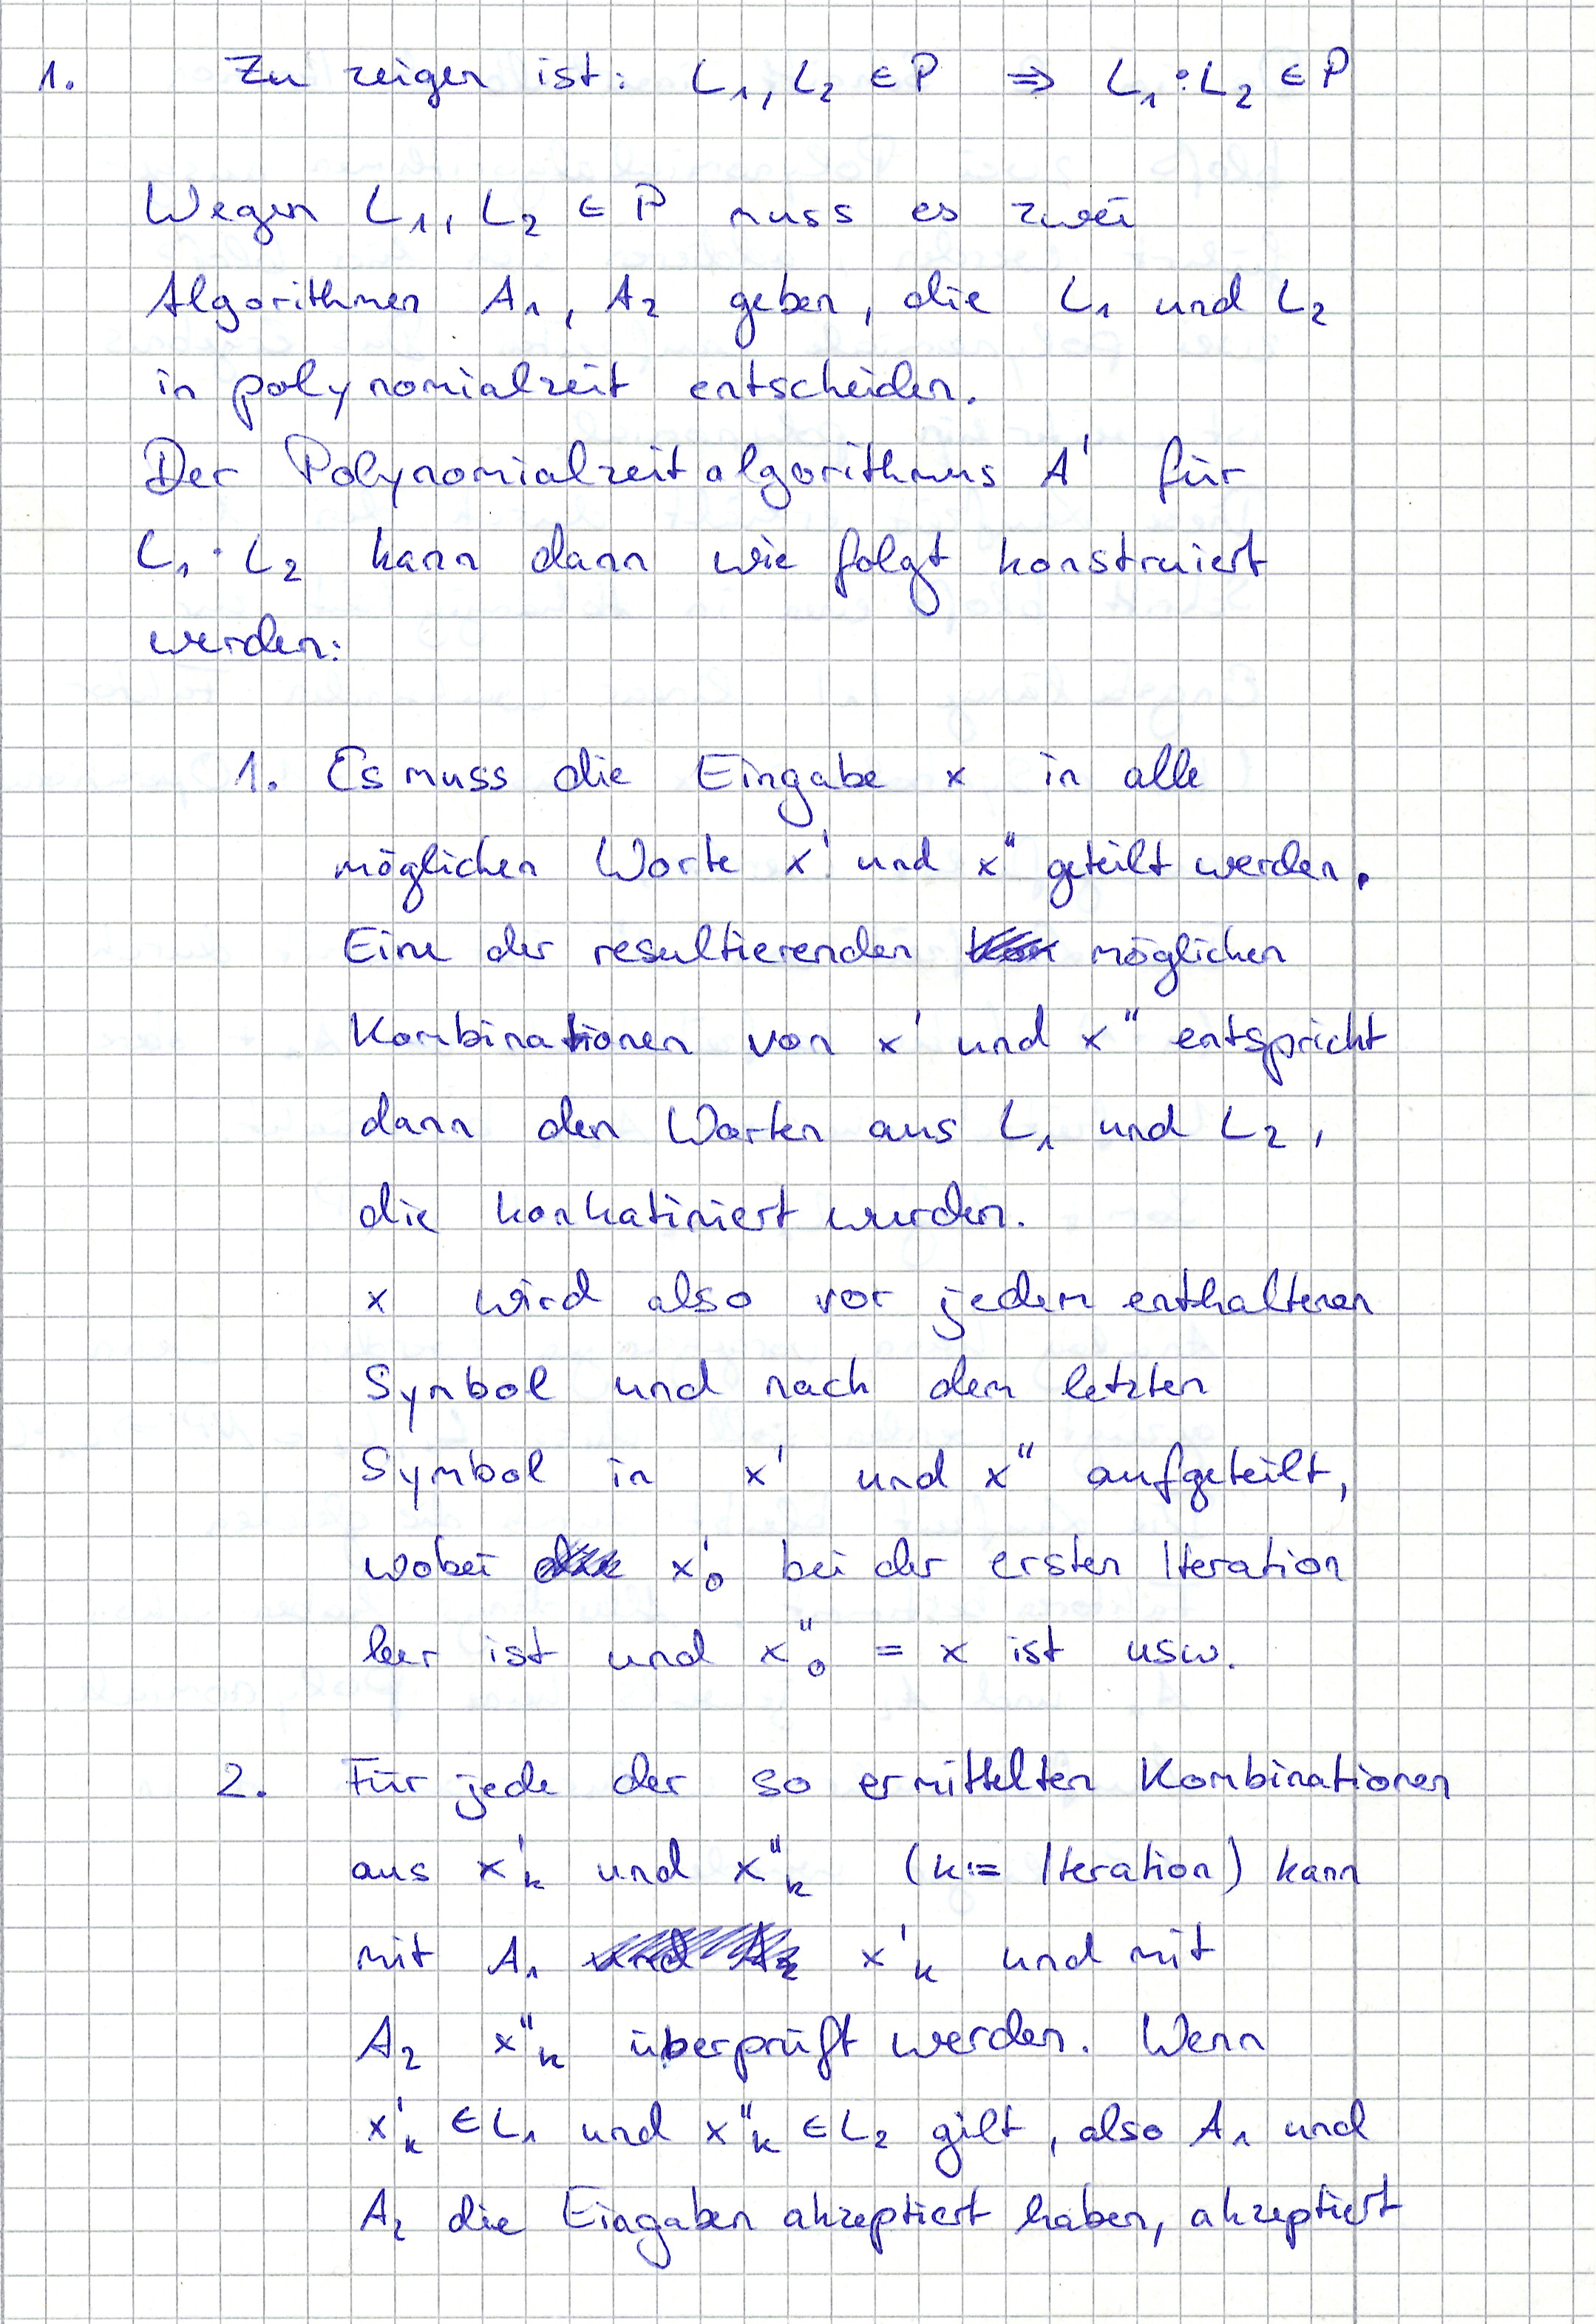
\includegraphics[width=1\textwidth]{a421-s1.png}
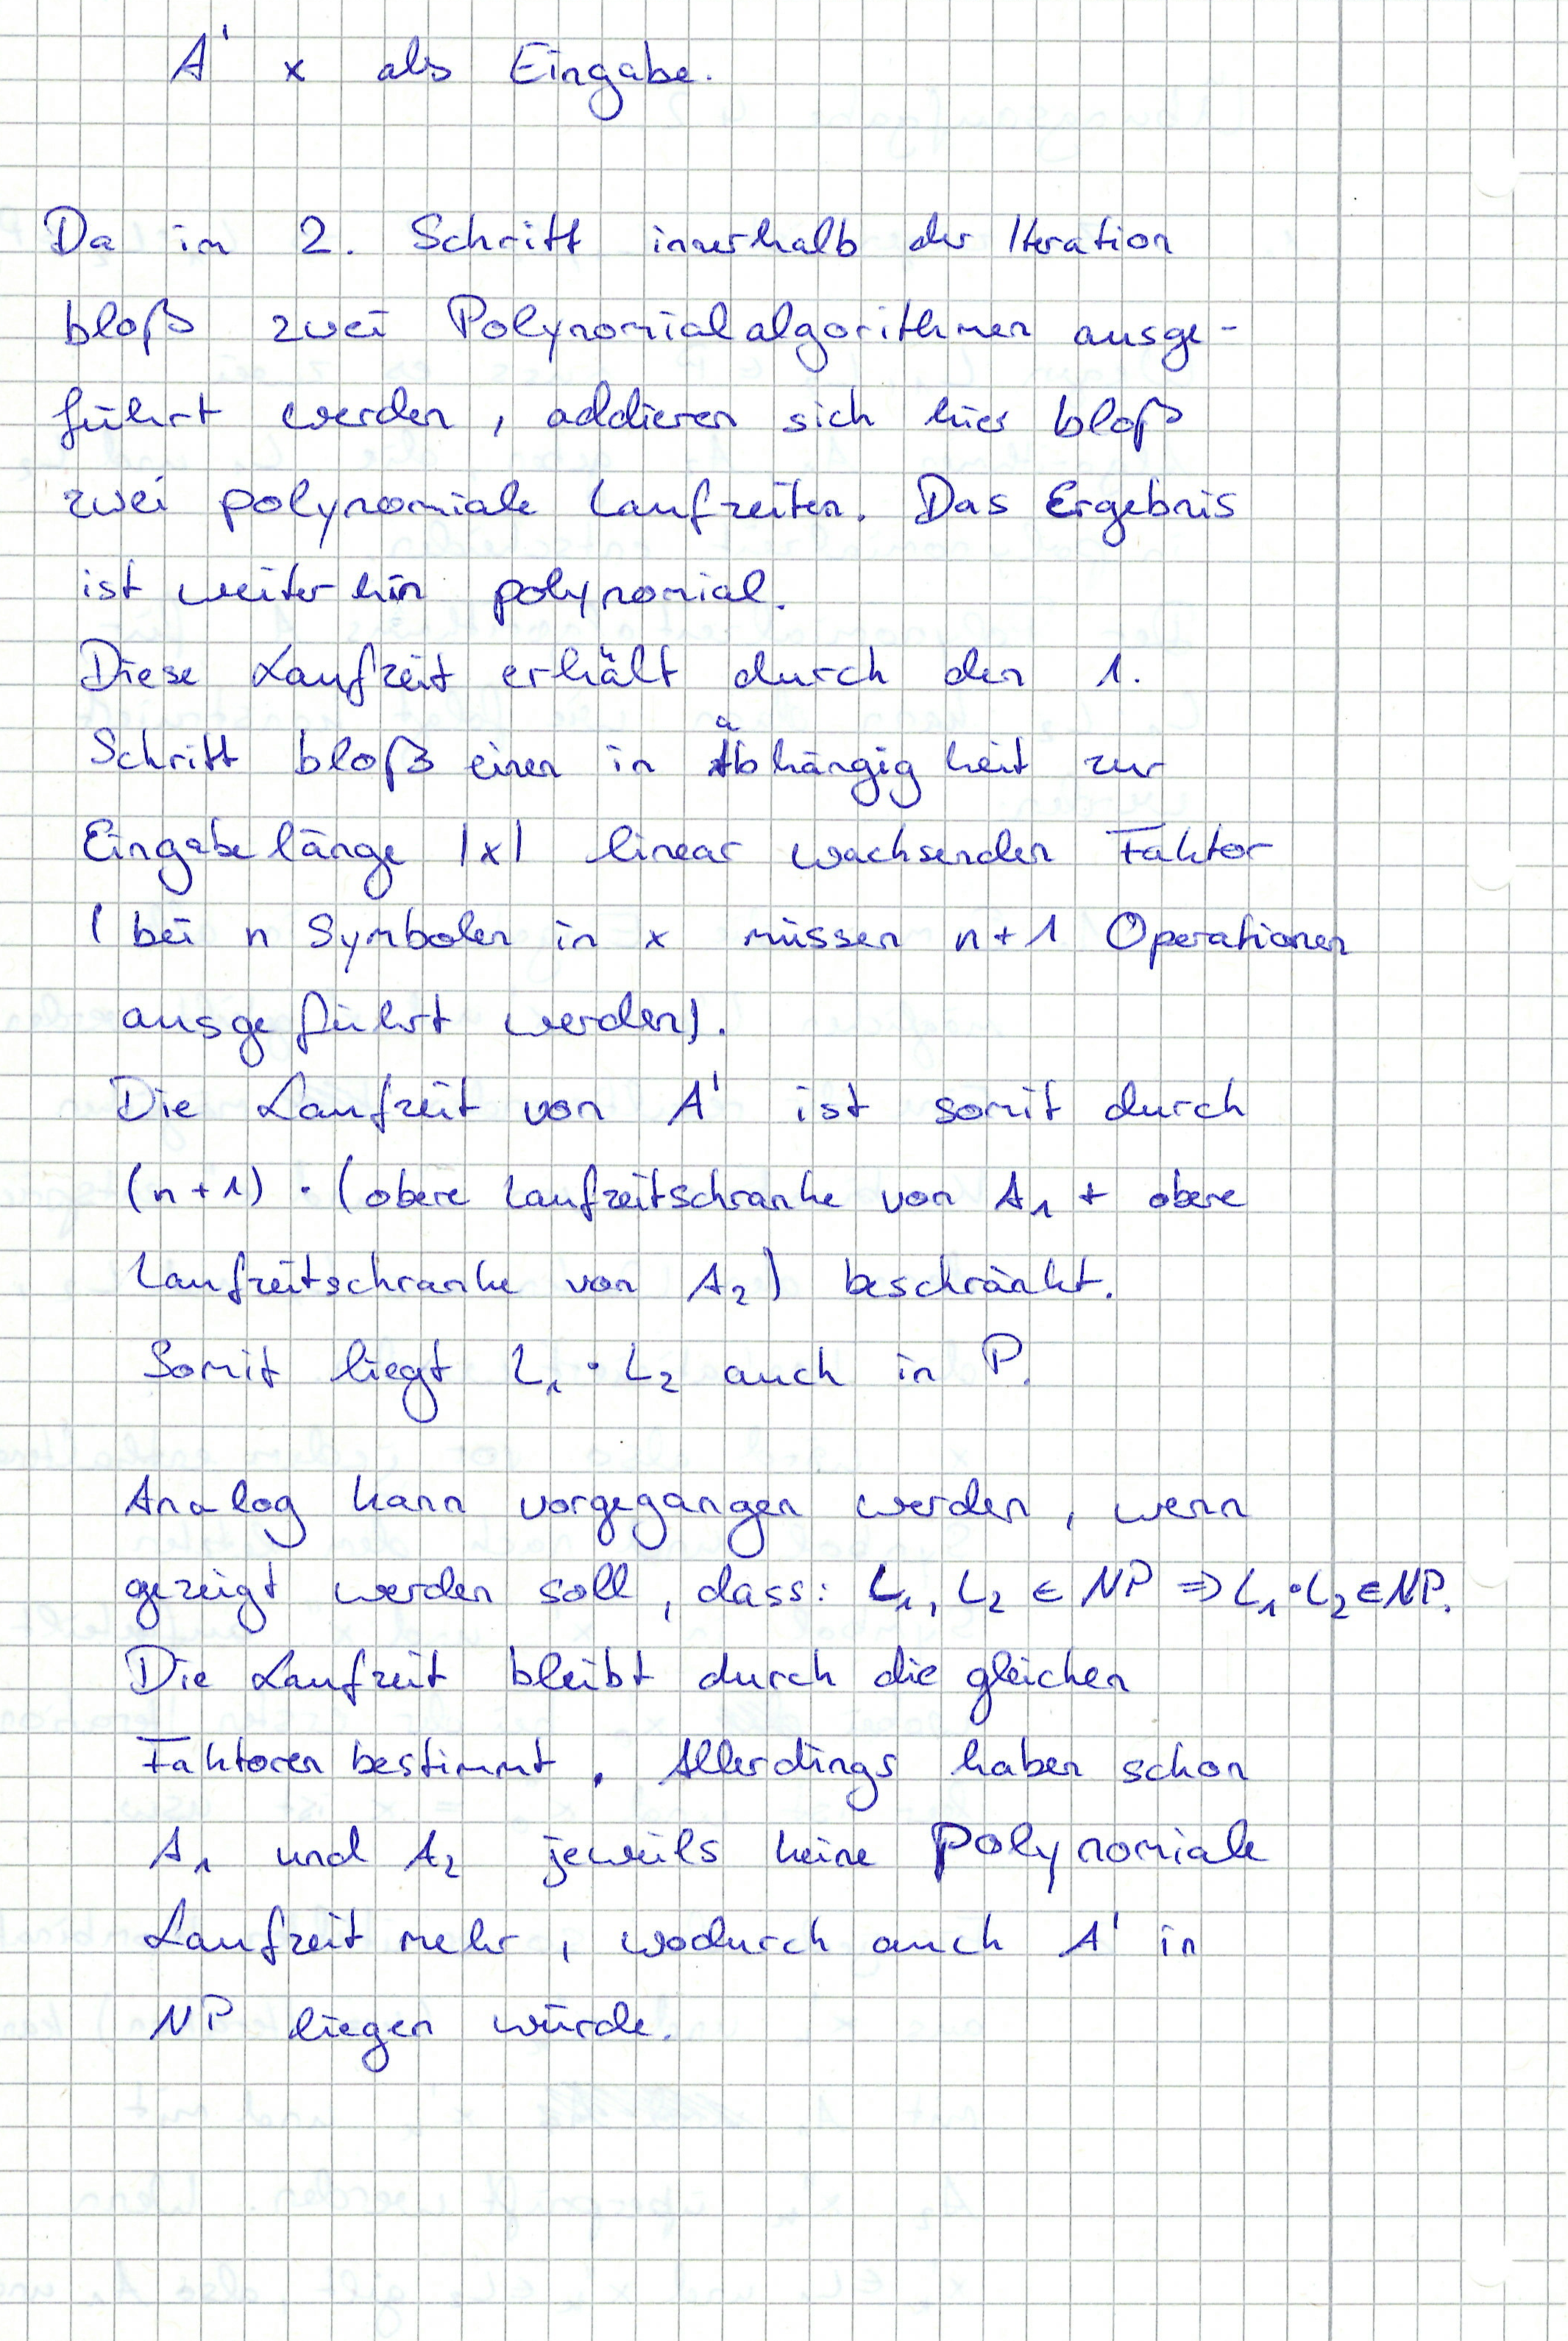
\includegraphics[width=1\textwidth]{a421-s2.png}

\subsection*{2.}

\subsection*{3.}
Die Klasse der NPC-vollständigen Probleme kann maximal alle Elemente der Klasse NP enthalten, da die erste Bedingung für NPC-vollständige Probleme besagt, dass sich das Problem in NP befinden muss.\\
Durch die Tatsache, dass NPC dadurch bestimmt ist, dass ein Algorithmus angegeben werden kann, der in polynomieller Laufzeit ein NP-Problem auf ein anderes reduzieren kann und wir hier ein NP-Algorithmus verwenden können, können wir mit genügend Zeit während der Reduktion jedes andere NP-Problem lösen.\\
Die Aussage gilt nicht für $\emptyset$, da die leere Sprache keine Eingaben akzeptiert.\\
Für $\Sigma^*$ gilt die Aussage nicht, da $\Sigma^*$ jede Eingabe akzeptiert, und deswegen kein Problem darauf reduziert werden kann.